Our first model of CLASP-driven root growth in \emph{A. thaliana} aims to qualitatively explain the phenomenon of cell zonation. A quantitative analysis of the differences in behaviour between the mutants is presented in Supplementary Figure \ref{sfig:data-trichoblast} and \ref{sfig:trichoblast-distribution}. In this model, each cell has a length $L$ which increases with time. Every cell also has a division level $D$. When $D > 1$, the cell divides into two cells with length $L / 2$ and division level $D = 0$. We model the changes in $L$ and $D$ over an arbitrary time scale using a number of assumptions described in the subsequent paragraphs.

\medskip

A cell can divide every $1/d_{0}$ time units at most. Cells must be at least $9\um$ long in order to divide (\cite{verbelen2006}). The cell division rate is inhibited by the length of the cell. By making this assumption, we treat cell length as a proxy for the levels of the various hormones that truly drive cell division. We also make the assumption that the CLASP-1 and BRIN-CLASP mutations do not modulate progress in the cell cycle directly. In other words, the $dD/dt$ equation is identical for the wild type, CLASP-1, and BRIN-CLASP models. This assumption may very well be incorrect, but it is sufficient to explain the observed data.

\medskip

Next, we let cells grow at a basal rate $g_{0}$. The BRIN-CLASP mutant and wild-type root have their basal growth rate decreased due to the presence of CLASP-driven microtubule bundles that run parallel to the axis of growth. Additionally, cells further from the QC grow at a faster rate due to the increased concentration of extracellular BL, which leads to higher levels of BES1 signalling. The CLASP-1 mutant and wild-type root have their position-dependent growth rate reduced by the fact that lower CLASP levels (compared to the BRIN-CLASP mutant) reduces the number of BRI1 receptors on the cell membrane which in turn leads to lower BES1 signalling levels. Cells also have a maximum size of $150 \mu m$ which comes from the "Sizer" model for cell differentiation presented by \cite{pavelescu2018} combined with observations from \cite{verbelen2006} and our experimental data. 

\medskip

To determine the exact equations used in the cell column model we need to take a closer look at the singalling network in the various mutants shown in Figure \ref{fig:mutant-diagram}. Observing the pathways in each mutant indicates that the CLASP level should be highest in the BRIN-CLASP mutant (since CLASP is not repressed by BES1), followed by the wild type, followed by the CLASP-1 mutant (which has no CLASP at all). Since CLASP promotes the recycling of BRI1 receptors, the number of receptors should also be highest in the BRIN-CLASP mutant, followed by the wild type, followed by the CLASP-1 mutant. Let $C_{\text{WT}}$ and $C_{\text{BC}}$ denote the level of CLASP in the wild type and BRIN-CLASP roots respectively. Similarly, define $R_{\text{WT}}$, $R_{\text{BC}}$, and $R_{\text{C1}}$ for the receptor levels. Using these variables we can define the equations for the model shown in Equation \eqref{column-equations}.

\begin{figure}
    \centering
    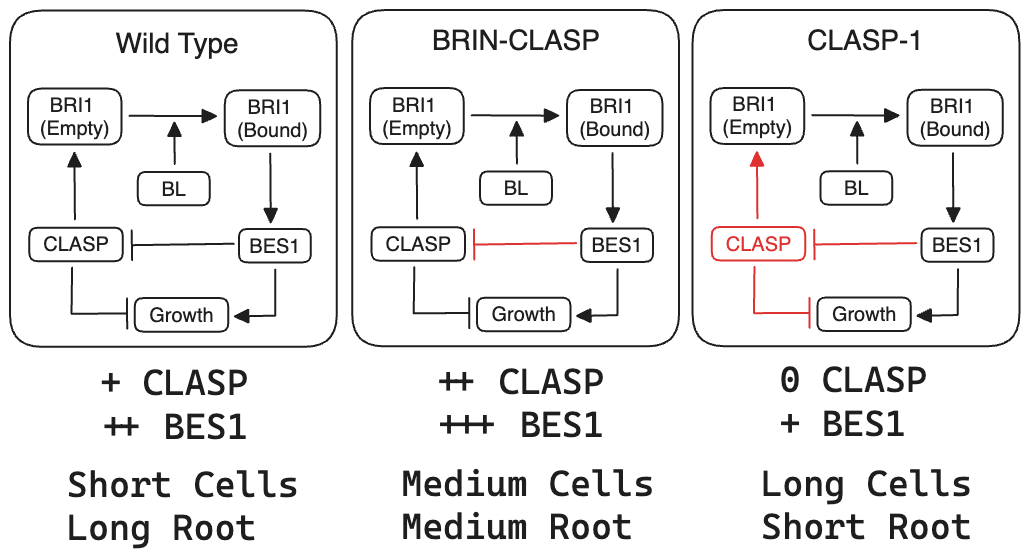
\includegraphics[width=13cm]{mutant-diagram.png}
    \caption{Signalling network in the wild type, BRIN-CLASP mutant, and CLASP-1 mutant. Red arrows denote signalling pathways that were removed due to the mutation.} 
    \label{fig:mutant-diagram}
\end{figure}


\begin{equation}
\label{column-equations}
\begin{aligned}
    &\frac{dL_{\text{C1}}}{dt} = ((g_{0} - 0) + R_{\text{C1}}P)L, &\frac{dD}{dt} = d_{0}\left( 1 - \frac{L^{n}}{d_{L}^{n} + L^{n}} \right)  \\[5pt]
    &\frac{dL_{\text{BC}}}{dt} = ((g_{0} - C_{\text{BC}}) + R_{\text{BC}}P)L, &\frac{dD}{dt} = d_{0}\left( 1 - \frac{L^{n}}{d_{L}^{n} + L^{n}} \right)  \\[5pt]
    &\frac{dL_{\text{WT}}}{dt} = ((g_{0} - C_{\text{WT}}) + R_{\text{WT}}P)L,  &\frac{dD}{dt} = d_{0}\left( 1 - \frac{L^{n}}{d_{L}^{n} + L^{n}} \right)
\end{aligned}
\end{equation}


\medskip

As discussed previously, these equations are subject to the restrictions $0 < C_{\text{WT}} < C_{\text{BC}}$ and $R_{\text{C1}} < R_{\text{WT}} < R_{\text{BC}}$. We ran the model with a time step $0.01$ for a period of $T = 500$ arbitrary units. The simulations were initialized with $10$ cells of length $7\um$. Parameters were fitted by hand to match an exponential curve fitted to experimentally observed data. The results of these simulations are shown in Figure \ref{fig:column-position-length}. For more information, see the supplementary figures in the appendix. The parameters used in all of the figures presented are shown in Table \ref{tab:cell-column-parameters} while information about division behaviour is shown in Table \ref{tab:cell-column-divisions}.


\begin{table}
    \begin{center}
        \begin{tabular}{ |c|c|c| }
        \hline
         Parameter & Units & Value \\
         \hline
         $g_{0}$ & $1/t$ & $0.02500$ \\ 
         $c_{\text{WT}}$ & $1/t$ & $0.01400$ \\ 
         $c_{\text{BC}}$ & $1/t$ & $0.02200$ \\ 
         $R_{\text{C1}}$ & $1/(\um \cdot t)$ & $0.00028$ \\ 
         $R_{\text{WT}}$ & $1/(\um \cdot t)$ & $0.00029$ \\ 
         $R_{\text{BC}}$ & $1/(\um \cdot t)$ & $0.00030$ \\ 
         $d_{0}$ & $D/t$ & $0.05000$ \\ 
         $d_{L}$ & $\um$ & $20.0000$ \\ 
         $n$ & $1$ & $20.0000$ \\ 
         \hline
        \end{tabular}
    \caption{Parameter values for cell column model.}
    \label{tab:cell-column-parameters}
    \end{center}
\end{table}

\begin{table}
    \begin{center}
        \begin{tabular}{ |c|c|c|c|c| } 
        \hline
        Model & Mean Div. & Median Div. & Max Div. & \# Divs.  \\
        \hline
        Wild Type & $158.51$ & $151.41$ & $344.34$ & $537$  \\
        BRIN-CLASP & $138.26$ & $131.49$ & $307.45$ & $523$  \\
        CLASP-1 & $96.28$ & $83.80$ & $241.98$ & $396$  \\
        \hline
        \end{tabular}
    \caption{Division behaviour in cell column models.}
    \label{tab:cell-column-divisions}
    \end{center}
\end{table}

\medskip

\begin{figure}
    \centering
    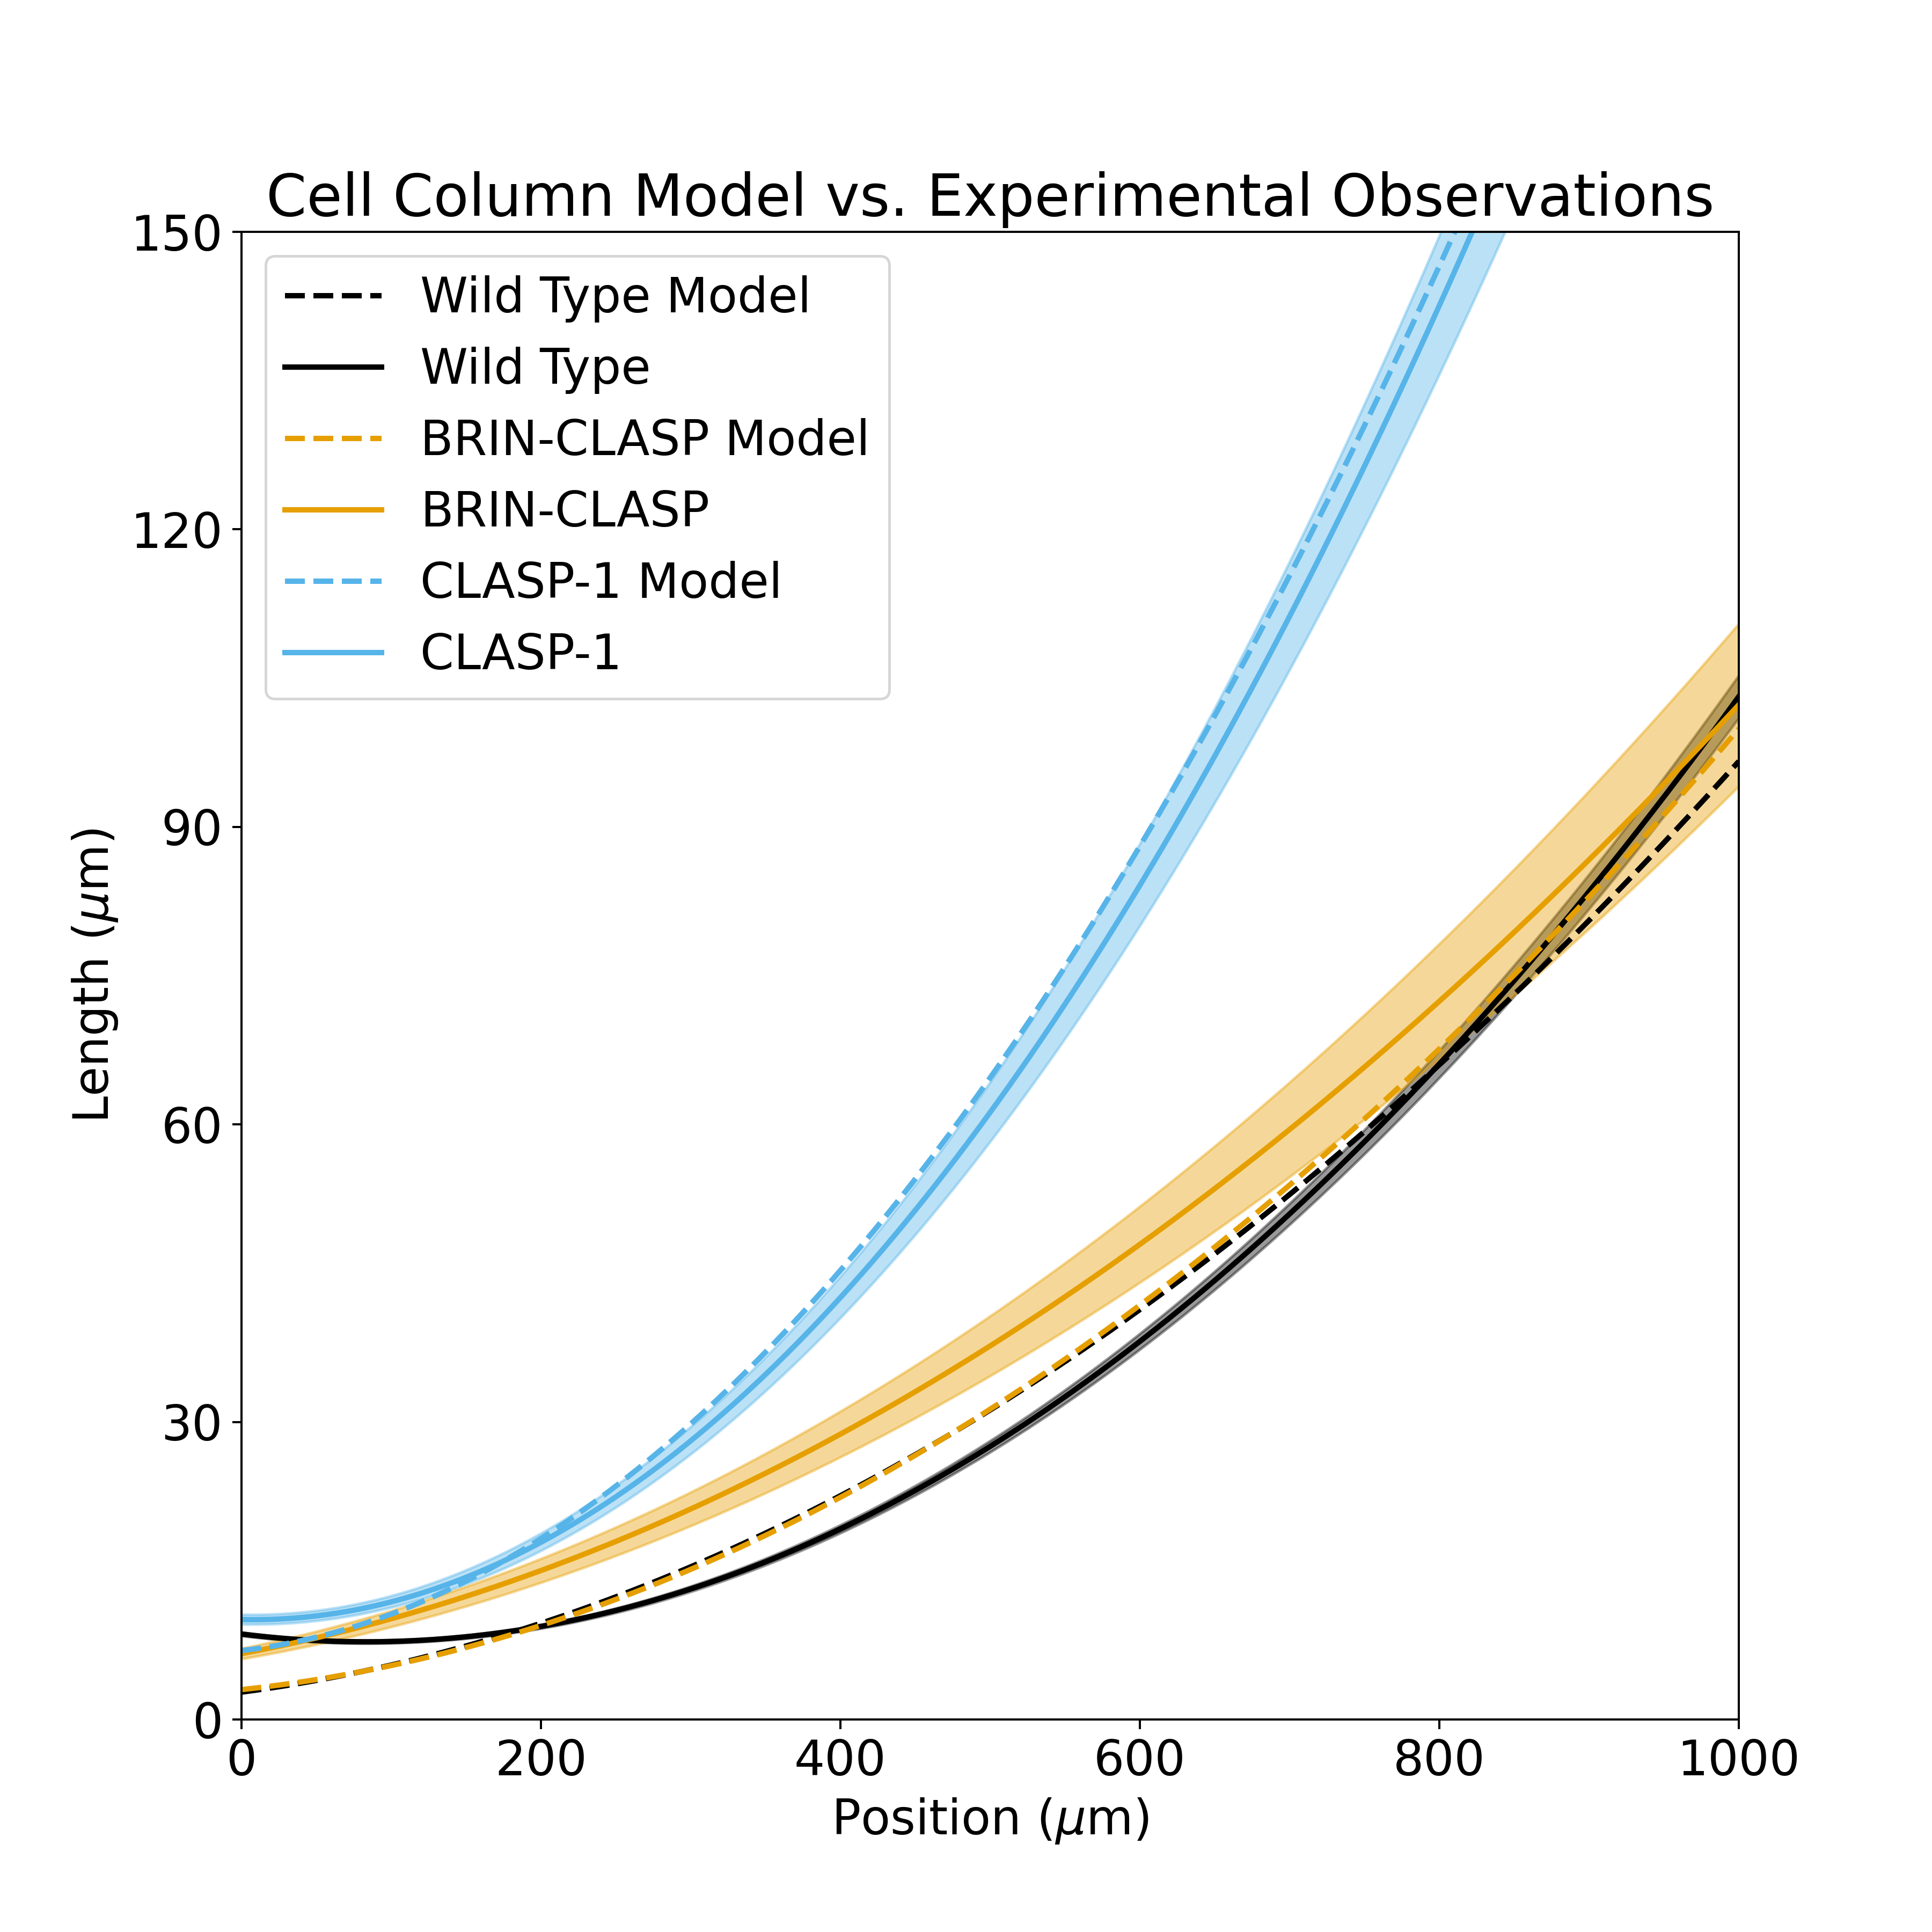
\includegraphics[width=13cm]{column-position-length.png}
    \caption{Position vs. length data from the model compared with experimental observations.}
    \label{fig:column-position-length}
\end{figure}

